% =============================================================================
% UFFIZI RL: TECHNICAL PROJECT PAPER
% Build from this directory with: pdflatex uffizi_paper.tex
% =============================================================================
\documentclass[11pt]{article}

\usepackage[a4paper,margin=2.25cm]{geometry}
\usepackage[T1]{fontenc}
\usepackage{lmodern}
\usepackage{microtype}
\usepackage{amsmath,amssymb,mathtools}
\usepackage{booktabs}
\usepackage{graphicx}
\usepackage{tabularx}
\usepackage{xcolor}
\usepackage[hidelinks]{hyperref}

\graphicspath{{../outputs/figures/}}

\setlength{\parindent}{1.15em}
\setlength{\parskip}{0.25em}
\renewcommand{\arraystretch}{1.18}

\newcommand{\R}{\mathbb{R}}
\newcommand{\E}{\mathbb{E}}
\newcommand{\Acal}{\mathcal{A}}
\newcommand{\ind}{\mathbb{1}}
\newcommand{\code}[1]{\texttt{\small #1}}
\newcommand{\fig}[1]{../outputs/figures/#1}
\newcolumntype{Y}{>{\raggedright\arraybackslash}X}
\newcolumntype{P}[1]{>{\raggedright\arraybackslash}p{#1}}

\title{\textbf{The Art of Queueing}\\
\large Reinforcement Learning for visitor flow at the Gallerie degli Uffizi in Florence}
\author{Marco Canal \and Michael Duarte Gon\c{c}alves \and Mircea-Adrian Guinea}
\date{Reinforcement Learning \\ June 2026}

\begin{document}
\maketitle

\begin{abstract}
The Uffizi Gallery makes congestion visible as a reinforcement-learning problem: capacity is not
scarce everywhere, but demand concentrates around Botticelli, Leonardo, Raphael-Michelangelo and
Caravaggio. We use two linked model layers. A minute-step agent-based simulator moves
heterogeneous visitors through the room graph and evaluates institutional interventions under a
revenue-preservation constraint. On top of those simulated crowds, RL agents solve the
visitor problem: when to stay, when to move and how far ahead, under RAMA, to reserve masterpiece
slots. The technical work is mostly formulation. Appreciation progress makes dwell decisions Markovian;
dense closing pressure prevents late trapping; reward design discounts congestion without making
masterpieces unattractive; action masks keep PPO on legal graph and booking-phase choices. In the
final simulator evaluation, the all-11 bundle raises completed welfare by 31\% at 5,000 visitors with
revenue essentially preserved. Five-seed MaskablePPO booking policies beat matched no-booking baselines
across profiles and crowds in every cell.
\end{abstract}

\section{Problem and Modeling Strategy}

The project starts from a common-pool resource problem. The Uffizi has enough total floor area to
serve many visitors, but visitor utility is degraded when a large share of demand arrives in the same
rooms at the same time. The clearest bottleneck is the Botticelli chain: rooms A11 and A12 lie on a
forced path and contain \emph{Primavera} and \emph{The Birth of Venus}. Leonardo and
Raphael/Michelangelo generate secondary peaks, while many other galleries remain underused. The RL
question is therefore not simply whether an agent can find a shortest path. It is whether a learner
can use time, route choice and reservation lead time to obtain a better visit than a fixed itinerary.

The implementation separates two decision problems. At the museum level, a minute-step simulator runs
a full day of heterogeneous visitors under the legal 900-person capacity constraint. Interventions
alter arrival curves, access rules, prices and secondary attractions; they are evaluated by whether
they improve welfare without making revenue politically infeasible. At the individual level, one
controlled visitor optimizes a visit conditional on either the status-quo or intervened crowd process.
In the status quo, the relevant action is mostly whether to remain in a room or continue along a
planned route. Under RAMA, the decisive action happens before entry: the visitor chooses how far in
advance to reserve masterpiece slots and must then pace the walk to reach those windows.

This distinction is important because the simulator and the RL agents answer different questions. The
simulator is the population transition model and produces the museum-wide welfare and revenue
statistics. The RL agents estimate an optimized individual ceiling under a fixed population process.
Collapsing the two would obscure the difference between evaluating an institutional intervention and
solving a single visitor's sequential decision problem.

\section{The Virtual Uffizi}

\subsection{Graph and calibration}

The physical museum is encoded as a directed graph $G=(V,E)$ built from the 98 rooms emphasized in the
slides plus operational nodes such as the entry, staircases, terrace and exit. Each room carries four
central attributes: cultural importance, dwell-time magnetism, legal or effective capacity and
section. Ordinary doors are represented bidirectionally; staircases and exit routes are directed. The topology is validated with structural invariants:
weak connectivity, reachability from the entry, reachability of an exit from every gallery, high
degree for the main corridor hubs and a forced Botticelli chain A10--A11--A12--A13.

Visitors arrive through 37 fifteen-minute entry slots with a broad morning-weighted envelope. The
simulator uses a one-minute time step, a 615-minute baseline day (08:15--18:30) and a final-entry
cutoff at 17:30. The full intervention scenario extends the day to 720 minutes. The population mix is
60\% Instagram tourists, 30\% normal tourists and 10\% art lovers. Instagram tourists concentrate on
famous rooms and the panoramic terrace, move quickly and are nearly crowd-indifferent. Normal
tourists visit the famous rooms plus a few canonical additions, such as the Tribune and Caravaggio.
Art lovers have heterogeneous taste vectors, longer dwell times, stronger crowd aversion and a higher
probability of accepting alternative routes.

The movement model is local and stochastic. Conditional on deciding to move, a visitor chooses among
neighbors with weights of the form
\[
w_{i\to j}=\max\{0.01,\; b_{\text{route}}(j)+b_{\text{importance}}(j)+b_{\text{crowd}}(j)\},
\qquad
P(i\to j)=\frac{w_{i\to j}}{\sum_{k\in N(i)} w_{i\to k}}.
\]
The route term rewards the next room on the recommended itinerary, the importance term pulls visitors
toward personally valuable rooms and the crowd term favors low-density alternatives only for
crowd-sensitive visitors or information-guided interventions. This expression is only the schematic
core. The executable simulator also contains policy-specific movement logic for RAMA slots, low-budget
exit seeking, tour groups, Caravaggio priority and masterpiece bypasses. The model is intentionally
behavioral rather than globally optimal: the simulator is designed to reproduce plausible crowd
pressure, while the controlled RL environments solve the individual optimization problem separately.

\subsection{Museum interventions}

The intervention catalog contains access controls, price instruments, time architecture and demand
redistribution. The slide language calls the final scenario ``all 11'' because the publication catalog
has eleven intervention specifications, including two pre-bundled combinations. In code, these
specifications are merged with last-write-wins semantics into nine distinct active switches: RAMA,
secondary-attractor enrichment, extended hours, dynamic pricing, resident annual pass expansion,
timed entry, quiet hours, a tour-group cap of 10 and a EUR150 group surcharge. A separate portfolio
optimizer screens interventions individually and then applies greedy forward selection followed by
one-step local search on a scalarized welfare/revenue objective. That optimization is useful as an
economic robustness check, but the RL booking agents are trained in the all-11 world because it is the
environment in which RAMA access is active and internally consistent.

\begin{table}[t]
\centering
\caption{Museum-wide simulator results: status quo versus the all-11 intervention world. Welfare is
total completed visitor welfare. Revenue is daily ticket revenue in EUR.}
\label{tab:museum-wide}
\begin{tabular}{lrrrrr}
\toprule
Crowd & Welfare base & Welfare int. & Gain & Revenue base & Revenue int. \\
\midrule
500   & 277,256   & 343,507   & +24\% & 11,542 & 11,317 \\
2,500 & 1,106,175 & 1,274,045 & +15\% & 56,604 & 56,544 \\
5,000 & 1,514,458 & 1,986,425 & +31\% & 96,502 & 94,792 \\
\bottomrule
\end{tabular}
\end{table}

Figure~\ref{fig:density} gives the corresponding spatial evidence. At the 5,000-visitor crowd,
Botticelli peak density falls from 1.82 to 1.00 and traffic is distributed over a longer operating
window. The intervention does not make the museum empty; rather, it keeps the highest-demand rooms
closer to usable capacity.

\begin{figure}[t]
\centering
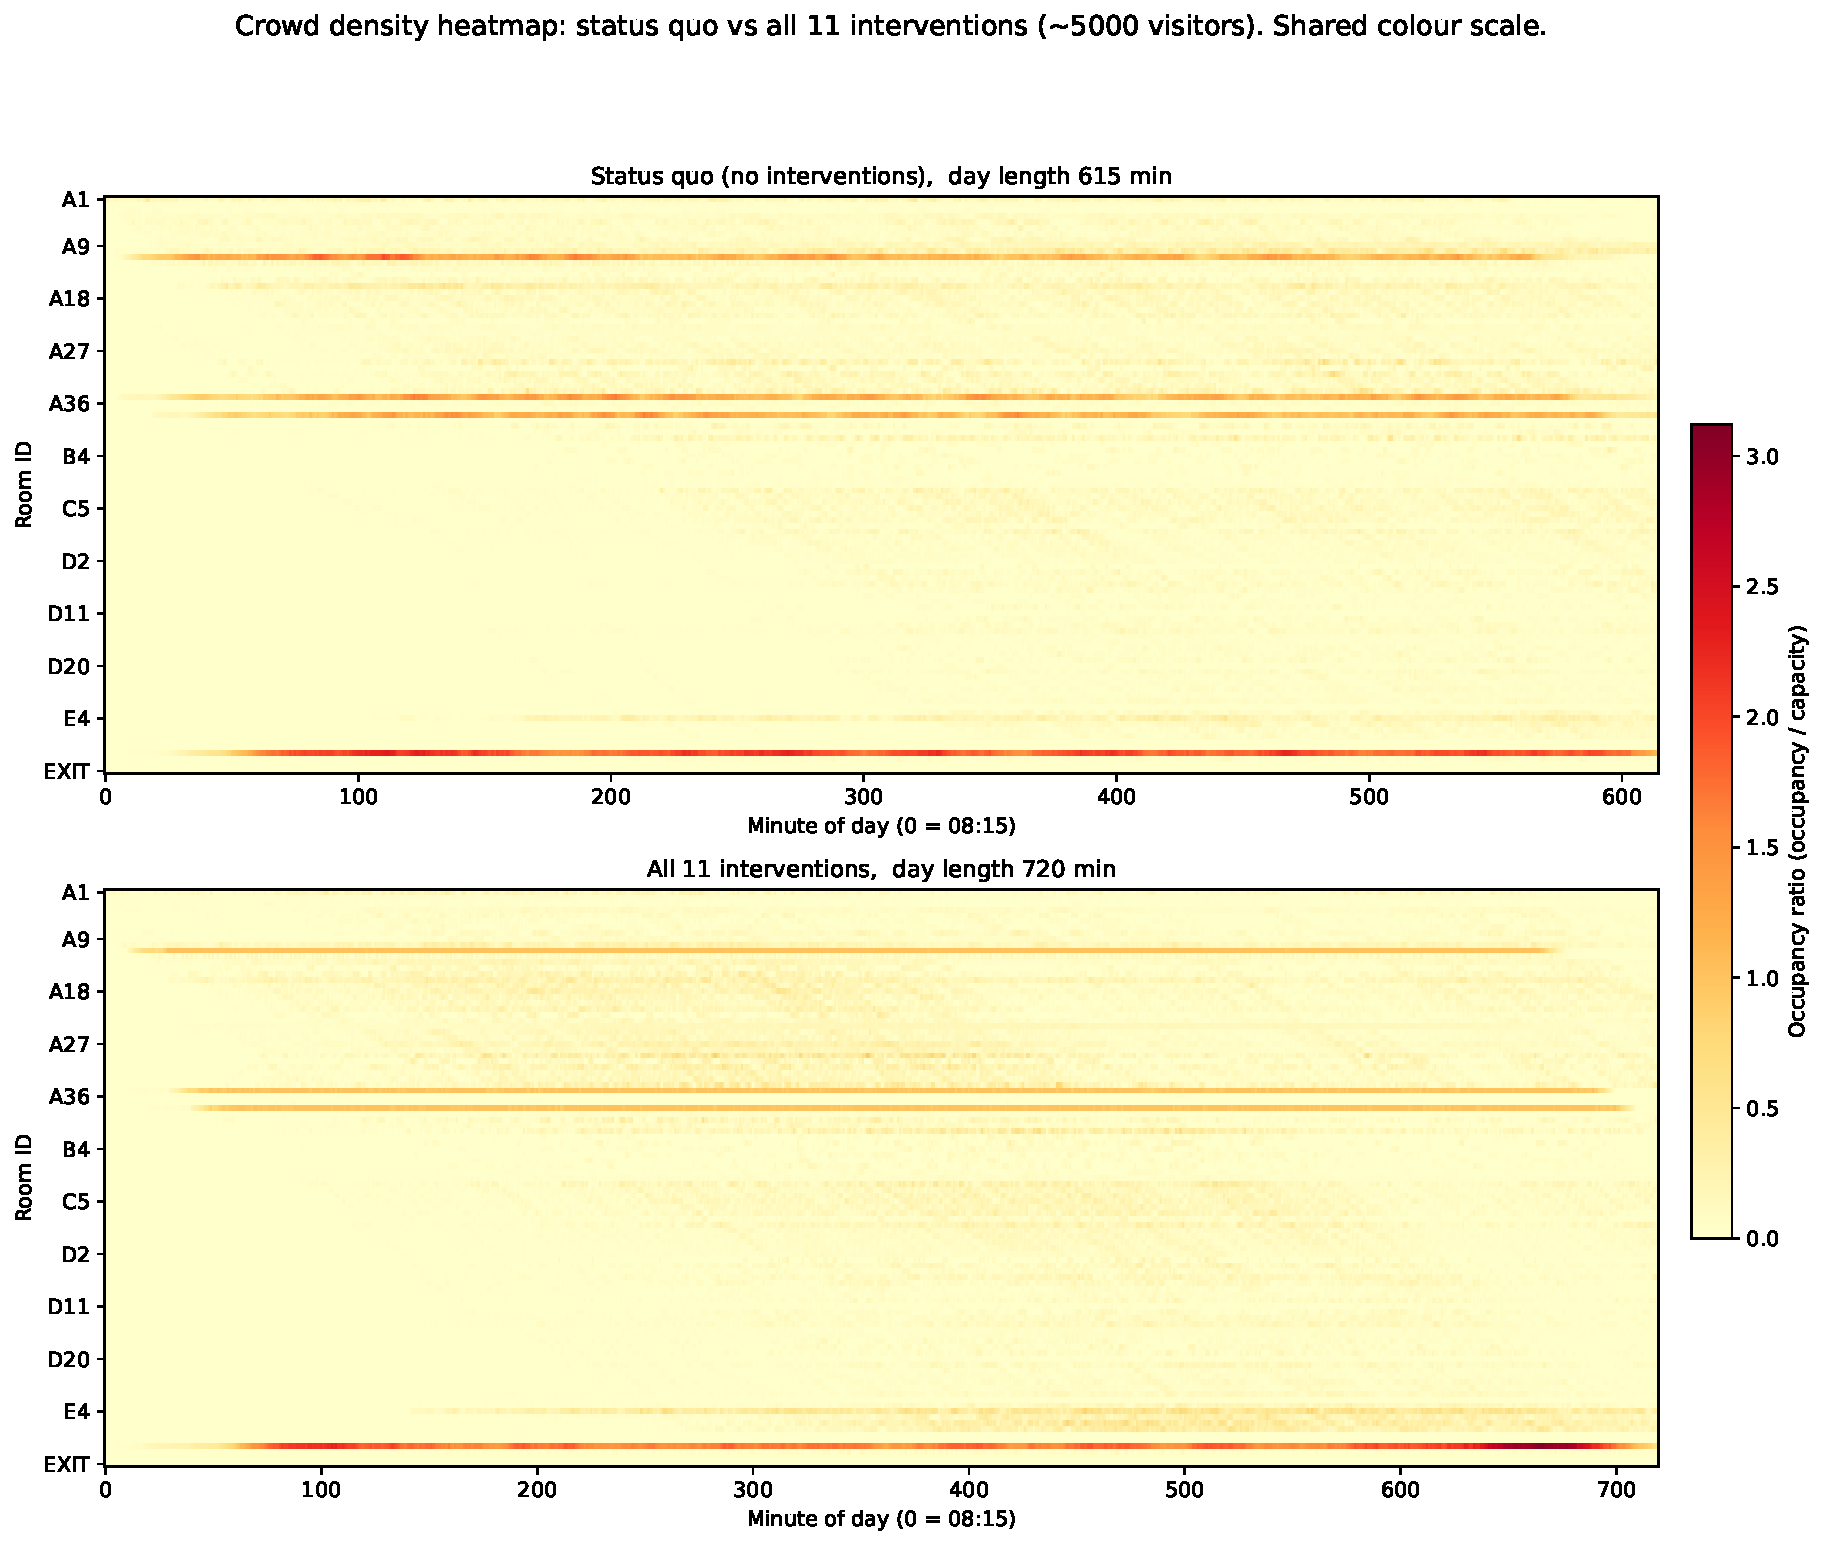
\includegraphics[width=\linewidth]{36_density_heatmap_intervened.pdf}
\caption{Crowd density under the status quo and under the full intervention bundle. The color scale is
shared, so cooling of the red bands corresponds to a real reduction in occupancy over capacity.}
\label{fig:density}
\end{figure}

\section{MDP Formulations}

All individual agents are standard discounted Markov decision processes
$\mathcal{M}=(\mathcal{S},\mathcal{A},P,r,\gamma)$, but the relevant state and action space change
with the decision problem. The implementation lesson is that algorithm choice was secondary to
specifying what the agent could observe and what decision it was actually allowed to make.

\begin{table}[t]
\centering
\small
\caption{The three MDP families used in the project.}
\label{tab:mdps}
\begin{tabularx}{\linewidth}{@{}P{0.16\linewidth}Y P{0.20\linewidth}P{0.17\linewidth}@{}}
\toprule
Setting & State & Action & Algorithms \\
\midrule
Toy museum &
Discrete 5-tuple: room, time bin, Botticelli crowd bin, Leonardo crowd bin, visited mask &
Stay or move to a neighbor &
Q-learning, Double-Q \\
Status-quo walk &
8 real features: drain, importance, density, on-target, plan share, time, egress, distance &
Stay or move on &
PPO, DQN \\
RAMA booking &
25 real features: booking phase, lead screen, held windows, check-ins, access read, arrival priors,
room tail &
Phase-dependent lead, commit, stay, move choices &
MaskablePPO, PPO, DQN \\
\bottomrule
\end{tabularx}
\end{table}

\subsection{Tabular proof of concept}

The toy museum has 12 rooms and deterministic crowd waves. It is small enough for a literal
action-value table. The state is
\[
s=(\text{room},t_{\text{bin}},c_{\text{Bott}},c_{\text{Leo}},m_{\text{visited}}),
\]
where $c_{\text{Bott}}$ and $c_{\text{Leo}}$ are four-level crowd bins and
$m_{\text{visited}}$ is a bitmask over must-see rooms. Q-learning applies the masked Bellman update
\[
Q(s,a)\leftarrow Q(s,a)+\alpha\Big[
r+\gamma\max_{a'\in \Acal(s')}Q(s',a')-Q(s,a)\Big],
\]
where $\Acal(s')$ contains only legal graph moves. The toy confirms the basic economic idea:
learning beats fixed rules because it discovers temporal arbitrage, visiting Botticelli off-peak
rather than mechanically following the route. Over the five reported training seeds, Q-learning
reaches $83.3\pm3.8$ mean return and Double-Q reaches $83.1\pm3.7$, while the handcrafted rules range
from $-72.0$ to $35.4$. The small Q versus Double-Q gap is not surprising: the toy is mostly
deterministic, so there is little noisy maximization bias for Double-Q to remove.

\subsection{Status-quo navigation}

The status-quo full-museum agent uses a planned-route wrapper. It does not choose arbitrary
neighboring rooms; instead, it decides whether to remain in the current target or continue to the next
room in the planned walk. This gives the booking agent a fair comparison: the baseline is optimized,
but it cannot use RAMA.
The observation vector is
\[
o_{\text{walk}}\in\R^8 =
(\text{drain},\text{importance},\rho,\text{on-target},\text{plan-share},t,\text{egress},
\text{distance-to-next}).
\]
The ``drain'' feature is crucial. Without an appreciation-progress state, the decision ``stay until
I have seen enough, then leave'' is partially observed; the same physical room and time could require
opposite actions depending on how long the visitor has already been absorbing the work.

\subsection{RAMA as a two-phase MDP}

The RAMA environment is the centerpiece. It wraps the same core museum reward, but changes the action
interface. Phase 1 is a booking screen: choose a lead time from
\[
\ell\in\{1,7,21,35\}\text{ days},
\]
then commit to masterpiece windows. Phase 2 is the walk, where the visitor stays or moves and must
arrive inside the booked windows. The 25-dimensional observation groups into (i) booking position,
(ii) slots open by lead, (iii) windows and check-ins held, (iv) access information for the current
room, (v) frozen expected arrival times and (vi) the local room tail from the walk baseline.

The simplified availability rule is crowd-dependent:
\[
\text{available}(g,\ell)=
\ind\left[\ell \ge L_{\max}\,p_g\,\frac{N_{\text{day}}}{2500}\right],
\]
where $p_g$ is the popularity of masterpiece group $g$ and $N_{\text{day}}$ is daily demand. This is
the mechanism that makes late booking fail on busy days. Importantly, the policy is not told ``book
early when busy.'' It only sees slot availability and downstream reward.

\section{Reward Engineering}

The deep agents share a core per-minute reward implemented in the full Uffizi environment:
\[
r_t =
r_{\text{art}}+r_{\text{time}}+r_{\text{close}}+r_{\text{complete}}
+r_{\text{bored}}+r_{\text{checkin}}+r_{\text{wait}}.
\]
The main term is art value with crowd discount and satiation:
\[
r_{\text{art}} =
I_i\,
\frac{1}{1+\alpha \rho_i^2}\,
\operatorname{clip}\!\left(\frac{D_i-e_i}{s},0,1\right),
\qquad
D_i=\max\{1,k_d(I_i-I_0)\}.
\]
Here $I_i$ is the visitor-specific room importance, $\rho_i$ is density over capacity, $e_i$ is
appreciation already extracted and $D_i$ is ideal dwell time. Appreciation accumulates more slowly in
crowded rooms, so congestion hurts twice: it lowers instantaneous utility and consumes more of the
fixed day.

The final reward is the result of several failed intermediate specifications. A purely terminal
penalty for not exiting produced an almost flat reward landscape and the agent often learned to
remain in one room. The fix was to replace that sparse penalty with a dense closing signal,
\[
r_{\text{close}}=-\kappa\max(0,d_{\text{exit}}+b-\tau),
\]
where $\tau$ is time left. This term creates a learnable slope toward the exit before closing, while
remaining inactive when the visitor still has enough slack to continue sightseeing.

Crowding also had to be handled conservatively. When congestion was penalized too harshly, the art
lover learned a degenerate policy that avoided crowded masterpieces altogether. The final full-museum
reward therefore has no separate explicit congestion penalty; density discounts art value smoothly
rather than dominating it, because a crowded Botticelli room should remain preferable to an empty
corridor. Similarly, strong boredom penalties encouraged loops because moving reset the local penalty.
The final reward relies primarily on satiation and a small step cost, with only a modest
post-satiation boredom term active in the booking wrappers.

RAMA adds a booking-phase reward:
\[
r_{\text{book}} =
-d_{\text{decline}}n_{\text{decline}}
-k_{\text{mm}}\sum_{g\in \mathcal{B}} |w_g-\hat t_g|
-d_{\text{noshow}}n_{\text{noshow}}.
\]
The mismatch term was the decisive booking-phase addition. It charges, immediately at commitment time,
the distance between the reserved window $w_g$ and a frozen expected arrival time $\hat t_g$. Without
this off-pace proxy, the cost of a bad reservation arrives hundreds of steps later, creating a severe
credit-assignment problem. We also encode ``books the three masterpieces'' as a visitor-type trait
(\code{allow\_decline=False}); otherwise the availability of a decline action creates a degenerate
solution in which the agent avoids delayed risk by reserving nothing.

\section{Algorithms and Masking}

The full museum is too large for a table. We use PPO-family actor-critic methods for the main agents
and DQN as the value-based control. PPO optimizes the clipped surrogate
\[
L^{\text{CLIP}}(\theta)=
\E_t\left[
\min\left(\rho_t\hat A_t,\,
\operatorname{clip}(\rho_t,1-\epsilon,1+\epsilon)\hat A_t\right)
\right],
\qquad
\rho_t=\frac{\pi_\theta(a_t\mid s_t)}
{\pi_{\theta_{\text{old}}}(a_t\mid s_t)}.
\]
DQN minimizes a squared Bellman error against a target network and replay buffer:
\[
L(\theta)=\E_{(s,a,r,s')\sim\mathcal{D}}
\left[
\left(r+\gamma\max_{a'}Q(s',a';\theta^-)-Q(s,a;\theta)\right)^2
\right].
\]

Action masking is the key implementation detail. In the full navigation environment, most graph-action
indices are illegal in most states. In the RAMA wrapper, the action space is smaller but still
phase-dependent: lead choices are legal on the booking screen, commit choices are legal at the
reservation step and stay/move choices are legal during the walk. MaskablePPO sets illegal logits to
$-\infty$ before the softmax:
\[
\pi_\theta(a\mid s)=
\frac{\exp(z_a)\ind[a\in\Acal(s)]}
{\sum_{b\in\Acal(s)}\exp(z_b)}.
\]
Invalid actions therefore receive exactly zero probability and zero gradient. Unmasked PPO must learn
legality indirectly by sampling illegal moves and paying penalties, which wastes data. In easy cells
the difference is small; in the packed tourist RAMA cell it is outcome-determining.

The PPO-family arms use Stable-Baselines3 MLP policies with two 128-unit hidden layers, learning rate
$3\times10^{-4}$, rollout length 2048, batch size 256, 10 epochs per update, GAE $\lambda=0.98$,
clip range 0.2 and entropy coefficient 0.01. The no-booking walk baselines train for 150k steps with
$\gamma=0.995$ for art lovers and $0.997$ for tourists. RAMA booking policies train for 100k steps
with $\gamma=0.999$, which keeps delayed reservation payoffs alive. DQN uses a 100k replay buffer,
target updates every 1000 steps, train frequency 4, learning starts at 2k steps and
$\varepsilon$-greedy exploration decaying from 0.30 to 0.05.

Training uses common random numbers for evaluation: competing policies are scored on the same fixed
crowd seeds, so differences are due to policies rather than lucky simulation noise. The figures in
this paper use five training seeds $\{1,3,7,42,202606\}$, each evaluated deterministically on six
fixed crowd seeds \code{900000}--\code{900005}. The repository also stores the selected single-model
deliverable evaluation in \code{results\_rl\_booking.json}; the figures use the five-reseed means
because they reveal instability rather than hiding it.

\section{Results}

\subsection{Booking policy}

Table~\ref{tab:booking} shows the individual RL result used in the figures. The baseline is the best
matched no-intervention walk. The intervened score is the MaskablePPO RAMA booking policy in the
all-11 world, averaged over five independent training seeds and six fixed evaluation seeds. The art
lover at the packed crowd is the one visibly unstable cell: four runs learn the intended 3/3 booking
pattern, while one run collapses, producing both the large standard deviation and the $2.6/3$ mean
check-in rate.

\begin{table}[t]
\centering
\caption{RAMA booking agent versus matched no-intervention walk baseline. Points are five-training-seed
means; parentheses report the standard deviation of the intervened arm.}
\label{tab:booking}
\begin{tabular}{llrrrr}
\toprule
Profile & Crowd & Baseline & RAMA & Gain & Check-ins \\
\midrule
Art lover & 500   & 5,112 & 7,113 (0)     & +39\% & 3.0/3 \\
Art lover & 2,500 & 4,780 & 6,167 (291)   & +29\% & 3.0/3 \\
Art lover & 5,000 & 4,010 & 4,800 (1,891) & +20\% & 2.6/3 \\
Tourist   & 500   & 2,694 & 3,686 (0)     & +37\% & 3.0/3 \\
Tourist   & 2,500 & 2,708 & 3,695 (0)     & +36\% & 3.0/3 \\
Tourist   & 5,000 & 2,680 & 3,685 (0)     & +38\% & 3.0/3 \\
\bottomrule
\end{tabular}
\end{table}

\begin{figure}[t]
\centering
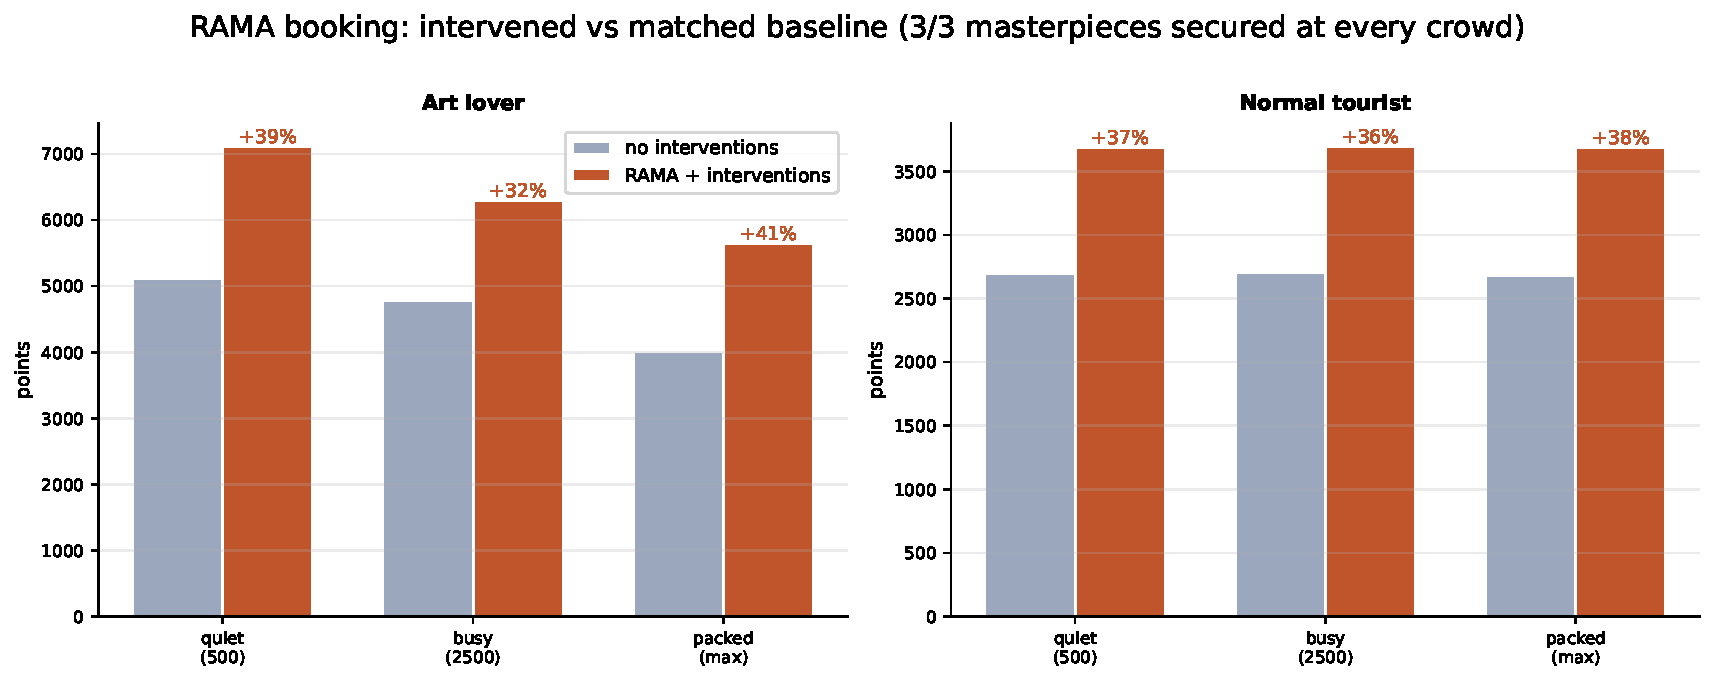
\includegraphics[width=\linewidth]{21_booking_grid.pdf}
\caption{RAMA booking gains over matched no-intervention walk baselines, reported as five-training-seed
means with standard-deviation bands. The grid is useful because it shows both profile heterogeneity and
crowd-level dependence.}
\label{fig:booking}
\end{figure}

The selected single-model deliverable run is stronger in the art-lover high-crowd cells, reaching
6,297 points at 2,500 visitors and 5,646 at 5,000 visitors in the six-seed deterministic evaluation.
The five-reseed table is more conservative and more informative technically, because it exposes the
rare but important failure mode. The tourist result is more stable: the shorter checklist and shorter
dwell targets make it easier to book the three windows and execute the route. The learned lead-time
curve still has the intended comparative static. Art lovers move from 7-day booking at the quiet crowd
to 35-day booking at busy and packed crowds; tourists stay at 7 days until the packed crowd, where the
reseeded curve moves later as well.

\subsection{Algorithm comparison}

Figure~\ref{fig:algorithms} isolates the algorithmic conclusion. MaskablePPO is best or tied in every
cell. Unmasked PPO collapses for the packed tourist in the intervened world, falling to 2,093 points
where MaskablePPO reaches 3,685. DQN is competitive in several easy tourist cells but crowd-fragile for
the art lover; under the no-intervention baseline, its art-lover return falls from 4,527 at the quiet
crowd to 2,044 at the packed crowd in the five-reseed mean.

\begin{figure}[t]
\centering
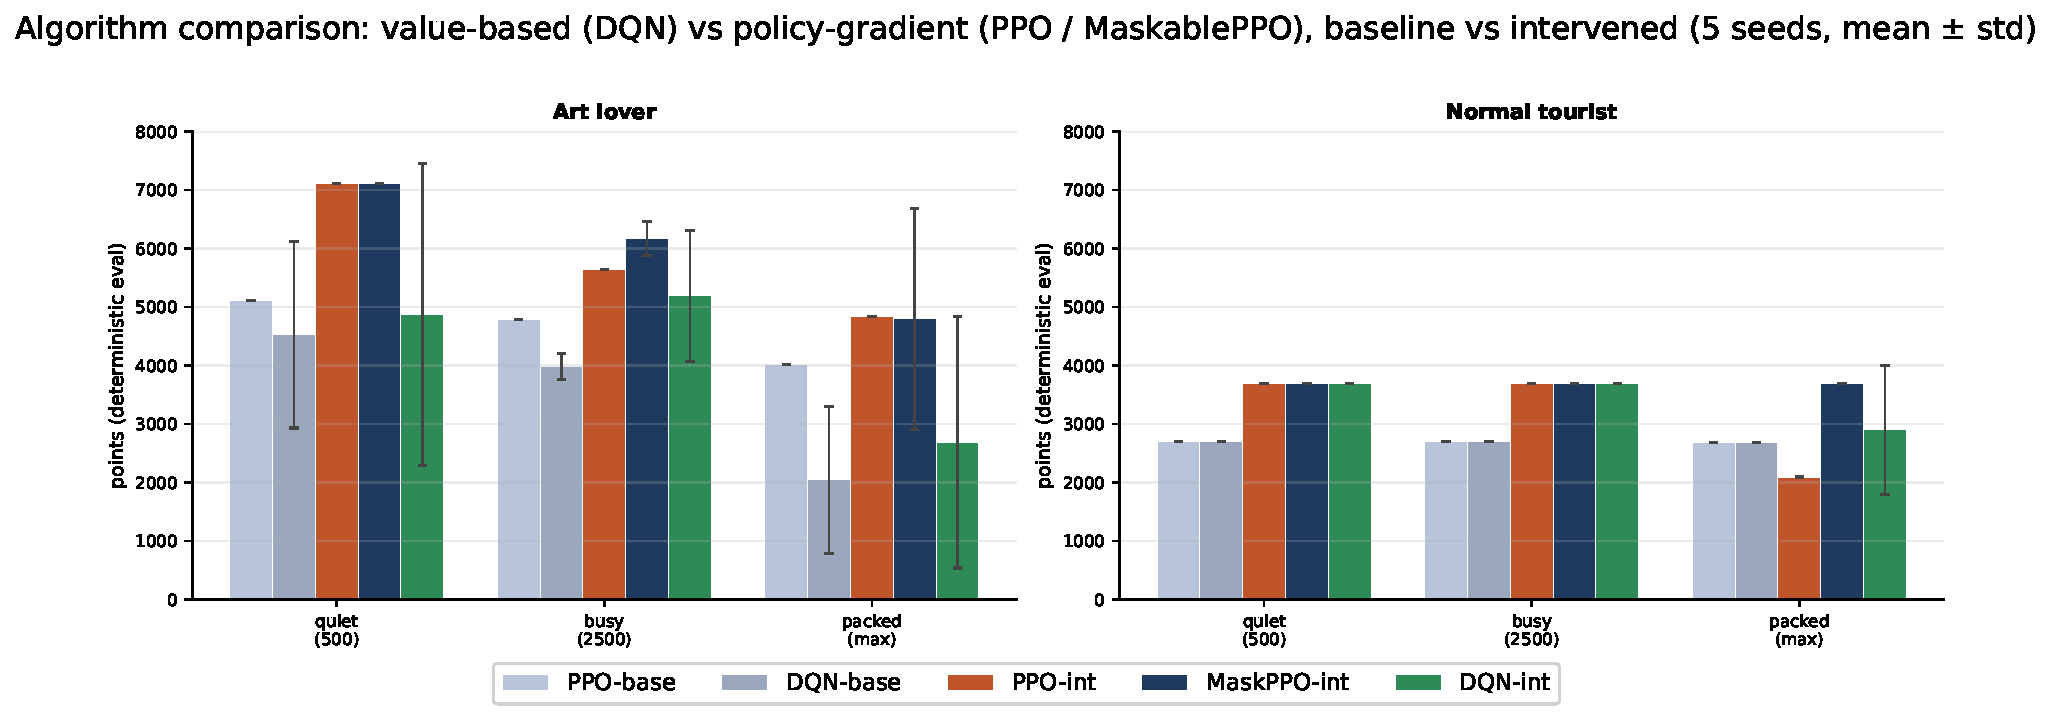
\includegraphics[width=\linewidth]{15_algorithm_comparison.pdf}
\caption{Algorithm comparison across profile and crowd cells. The dark-blue bars are MaskablePPO. The
gap to unmasked PPO at the packed tourist cell is the cleanest empirical evidence for action masking.}
\label{fig:algorithms}
\end{figure}

This pattern is consistent with the algorithms' failure modes. DQN inherits a maximization step over
noisy value estimates, the same issue that motivates Double-Q in the tabular setting. PPO avoids that
particular max-over-actions target, but unmasked PPO still spends exploration budget discovering
actions that are impossible in the current graph or booking phase. MaskablePPO removes that burden by
matching the policy support to the legal action set at every minute.

\section{Limitations}

The model is only as good as its calibration. Room topology and opening hours are grounded in public
sources and the official floor plan, but several behavioral parameters are explicit assumptions:
the exact 60/30/10 profile mix, heterogeneity scale, willingness-to-pay elasticity and intervention
compliance rates. The results should therefore be read as a controlled simulation study, not as a
claim that the real Uffizi would mechanically realize the same percentages.

There is also a reward-design limitation. We use a consistent welfare proxy, but museum experience is
not a single scalar. The reward values art exposure, crowd comfort, completion and timely exit; it
does not directly model learning, fatigue psychology, social groups, fairness constraints, or curatorial
goals beyond room importance and enrichment. Finally, the learned policies depend on the observation
shape. Changing the 8-dimensional walk state or 25-dimensional RAMA state invalidates the saved models
and requires retraining.

\section{Conclusion}

The project's main technical lesson is that useful learning required the right abstraction of the
decision problem. The status-quo visitor mostly faces a walking and dwell-time problem. The intervened
visitor faces a reservation problem with delayed payoffs, irreversible commitments and legality
constraints. Once the MDP exposes those variables, MaskablePPO learns the intended policy: reserve
masterpieces early, reserve even earlier on crowded days and pace the visit to collect the booked
windows.

At the museum level, the all-11 intervention world reduces the worst density bands and raises completed
welfare by 31\% at the 5,000-visitor crowd while preserving revenue. At the individual level, the RAMA
agent improves over optimized no-intervention baselines for both profiles and all crowds, with one
high-variance art-lover cell that is visible only when the five training reseeds are kept. The most
robust engineering takeaway is action masking: respecting the legal action set matters more than extra
tuning once the environment becomes hard.

\begin{thebibliography}{9}

\bibitem{attanasio2022}
Attanasio, A., et al. (2022).
\newblock Visitors flow management at Uffizi Gallery.
\newblock \emph{Information Technology \& Tourism}, 24(3), 409--434.

\bibitem{centorrino2021}
Centorrino, P., et al. (2021).
\newblock Managing crowded museums: Visitors flow measurement, analysis, modeling and optimization.
\newblock \emph{Journal of Computational Science}, 53, 101357.

\bibitem{mnih2015}
Mnih, V., et al. (2015).
\newblock Human-level control through deep reinforcement learning.
\newblock \emph{Nature}, 518, 529--533.

\bibitem{schulman2017}
Schulman, J., Wolski, F., Dhariwal, P., Radford, A. and Klimov, O. (2017).
\newblock Proximal policy optimization algorithms.
\newblock arXiv:1707.06347.

\bibitem{sutton2018}
Sutton, R. S. and Barto, A. G. (2018).
\newblock \emph{Reinforcement Learning: An Introduction}.
\newblock MIT Press, 2nd edition.

\bibitem{veron1983}
Veron, E. and Levasseur, M. (1983).
\newblock \emph{Ethnographie de l'exposition}.
\newblock Bibliotheque publique d'information, Centre Georges Pompidou.

\end{thebibliography}

\end{document}
